\section{Trigonometria}

\smallskip{\centering
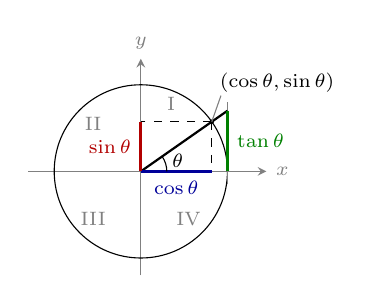
\begin{tikzpicture}[scale=0.55, >=stealth]
  \draw[->, gray] (-2.6,0) -- (2.9,0) node[right] {\scriptsize $x$};
  \draw[->, gray] (0,-2.4) -- (0,2.6) node[above] {\scriptsize $y$};
  \draw (0,0) circle (2);
  \draw[gray] (2,-0.3) -- (2,1.6);
  \draw[thick] (0,0) -- (2,1.400);
  \draw[dashed] (1.638,1.147) -- (1.638,0);
  \draw[blue!60!black, very thick] (0,0) -- (1.638,0);
  \node[blue!60!black, below] at (0.82,0) {\scriptsize $\cos\theta$};
  \draw[dashed] (1.638,1.147) -- (0,1.147);
  \draw[red!70!black, very thick] (0,0) -- (0,1.147);
  \node[red!70!black, left] at (0,0.57) {\scriptsize $\sin\theta$};
  \draw[green!50!black, very thick] (2,0) -- (2,1.400);
  \node[green!50!black, right] at (2,0.7) {\scriptsize $\tan\theta$};
  \draw (0.6,0) arc (0:35:0.6);
  \node at (0.85,0.25) {\scriptsize $\theta$};
  \fill (1.638,1.147) circle (1.5pt);
  \draw[gray] (1.638,1.147) -- (1.85,1.75);
  \node[anchor=south west, inner sep=1pt] at (1.75,1.75) {\scriptsize $(\cos\theta, \sin\theta)$};
  \node[gray] at (0.7,1.55) {\scriptsize I};
  \node[gray] at (-1.1,1.1) {\scriptsize II};
  \node[gray] at (-1.1,-1.1) {\scriptsize III};
  \node[gray] at (1.1,-1.1) {\scriptsize IV};
\end{tikzpicture}
\par}\smallskip

O ponto do círculo de raio $1$ no ângulo $\theta$ (anti-horário a partir do eixo $x$) é $(\cos\theta, \sin\theta)$, e
$\tan\theta = \sin\theta / \cos\theta$ é a altura onde a reta pela origem corta $x = 1$. Também
$\cot = 1 / \tan$, $\sec = 1 / \cos$ e $\csc = 1 / \sin$. No 1º quadrante tudo é positivo, no 2º só $\sin$, no 3º só
$\tan$ e no 4º só $\cos$.

\smallskip{\centering\renewcommand{\arraystretch}{1.35}
\begin{tabular}{c|cccccc}
  $\theta$ & $0$ ($0^\circ$) & $\frac{\pi}{6}$ ($30^\circ$) & $\frac{\pi}{4}$ ($45^\circ$) & $\frac{\pi}{3}$ ($60^\circ$) & $\frac{\pi}{2}$ ($90^\circ$) & $\pi$ ($180^\circ$) \\ \hline
  $\sin$ & $0$ & $\frac12$ & $\frac{\sqrt2}{2}$ & $\frac{\sqrt3}{2}$ & $1$ & $0$ \\
  $\cos$ & $1$ & $\frac{\sqrt3}{2}$ & $\frac{\sqrt2}{2}$ & $\frac12$ & $0$ & $-1$ \\
  $\tan$ & $0$ & $\frac{\sqrt3}{3}$ & $1$ & $\sqrt3$ & -- & $0$
\end{tabular}
\par}\smallskip

\subsection*{Identidades}

\begin{itemize}
  \item $\sin^2 x + \cos^2 x = 1$, $\sin(-x) = -\sin x$ e $\cos(-x) = \cos x$.
  \item $\sin(a \pm b) = \sin a \cos b \pm \cos a \sin b$ e $\cos(a \pm b) = \cos a \cos b \mp \sin a \sin b$.
  \item $\sin 2x = 2 \sin x \cos x$ e $\cos 2x = \cos^2 x - \sin^2 x$.
\end{itemize}

\subsection*{Triângulo}

Com o lado $a$ oposto ao ângulo $A$ (e o mesmo para $b$ e $c$), $s = \frac{a + b + c}{2}$ o semiperímetro, $S$ a área,
$R$ o raio do círculo circunscrito e $r$ o do inscrito:
\begin{itemize}
  \item \textbf{Ângulos:} $A + B + C = \pi$, e com $C = 90^\circ$ vale Pitágoras, $a^2 + b^2 = c^2$.
  \item \textbf{Lei dos senos:} $\frac{a}{\sin A} = \frac{b}{\sin B} = \frac{c}{\sin C} = 2R$.
  \item \textbf{Lei dos cossenos:} $a^2 = b^2 + c^2 - 2bc \cos A$, então $\cos A = \frac{b^2 + c^2 - a^2}{2bc}$.
  \item \textbf{Área:} $S = \frac{1}{2} ab \sin C = \sqrt{s(s - a)(s - b)(s - c)}$ (Heron) $= \frac{abc}{4R} = rs$.
  \item \textbf{Raios:} $r = \frac{S}{s}$ e $R = \frac{abc}{4S}$.
  \item \textbf{Altura e mediana de $a$:} $h_a = \frac{2S}{a}$ e $m_a = \frac{1}{2}\sqrt{2b^2 + 2c^2 - a^2}$.
\end{itemize}

\subsection*{Funções inversas}

\texttt{atan2(y, x)} é o ângulo do vetor $(x, y)$ em $[-\pi, \pi]$, com o quadrante certo. Em \texttt{acos} e
\texttt{asin}, um valor como $1 + 10^{-16}$ dá \texttt{NaN}, então use \texttt{acos(clamp(x, -1.0, 1.0))}.
